\documentclass[a5paper,10pt]{article}

%\usepackage{showframe}

\usepackage[utf8]{inputenc}
\usepackage[spanish]{babel}
\usepackage[T1]{fontenc}
\usepackage[]{times}
\usepackage[linkcolor=blue,urlcolor=blue,colorlinks=true]{hyperref}
\usepackage{graphicx}
%\usepackage{subcaption}
\usepackage{listingsutf8}
\usepackage[dvipsnames]{xcolor}

\addtolength{\voffset}{-2cm}
\addtolength{\textheight}{4cm}

% Se incluyen formatos redifinidos para paquete listings
\renewcommand{\lstlistingname}{Código}

% Código fuente tipo consola (shell)
\lstdefinestyle{consola}{
  backgroundcolor=\color{black},
  belowcaptionskip=1\baselineskip,
  frame=,
  xleftmargin=\parindent,
  language=bash,
  basicstyle=\footnotesize\ttfamily\color{white},
  commentstyle=\itshape\color{purple!40!black}
}

% Código fuente tipo XML
\lstdefinestyle{miXML}{
    language=XML,
    morekeywords={classpath,classpathentry},
    basicstyle=\footnotesize\ttfamily\color{white},
    identifierstyle=\footnotesize\ttfamily\color{SkyBlue},
    commentstyle=\itshape\color{green!80},
    stringstyle=\color{Apricot},
    keywordstyle=\color{cyan!90},
    breaklines=true,
    backgroundcolor=\color{black},
    belowcaptionskip=1\baselineskip,
    rulecolor=\color{black},
    frame=trbl,
    xleftmargin=\parindent
}

% Código fuente tipo consola (json mejor)
% \lstdefinelanguage{json}{
\lstdefinestyle{miJSON}{
  string=[b][\color{Apricot}]",
  comment=[l][\itshape\color{green!80}]//,
  morecomment=[s][\color{SkyBlue}]{:}{,},
  morekeywords={true,false},
  basicstyle=\footnotesize\ttfamily\color{white},
  keywordstyle=\footnotesize\ttfamily\bfseries\color{purple!60},
  backgroundcolor=\color{black},
  breaklines=true,
  belowcaptionskip=1\baselineskip,
  rulecolor=\color{black},
  frame=trbl,
  xleftmargin=\parindent
}

% Código fuente ANTLR
\lstdefinestyle{miANTLR}{
    language=Java,
    basicstyle=\footnotesize\ttfamily\color{black},
    identifierstyle=\footnotesize\ttfamily\color{blue},
    commentstyle=\itshape\color{green},
    stringstyle=\color{red},
    keywordstyle=\bfseries\color{blue},
    keywords={grammar,\@header,fragment},
    morecomment=[s][\color{red!80!yellow}]{[}{]},
    moredelim=*[s][\ttfamily\itshape\footnotesize]{\{}{\}},
    breaklines=true,
    backgroundcolor=\color{black!5},
    belowcaptionskip=1\baselineskip,
    rulecolor=\color{black},
    frame=single,
    numbers=left,
    numbersep=5pt,
    numberstyle=\scriptsize\ttfamily,
    xleftmargin=\parindent
}


\lstdefinestyle{editor}{
  backgroundcolor=\color{black!5},
  belowcaptionskip=1\baselineskip,
  frame=single,
  numbers=left,
  xleftmargin=\parindent,
  language=bash,
  basicstyle=\footnotesize\ttfamily\color{black},
  commentstyle=\itshape\color{purple!40!black},
}




\author{Maximiliano A. Eschoyez}
\title{ANTLR en Visual Studio Code}
\date{2021}

\begin{document}
%\ebook
\maketitle

%\tableofcontents

\begin{abstract}
	Esta guía tiene como fin explicar la utilización de ANTLR en la IDE Visual Studio Code con Maven como gestor de proyecto.  Se explican los pasos mínimos desde la instalación de ANTLR Java hasta la compilación de código fuente y la generación de diferentes gráficos de análisis.
\end{abstract}

\section{Preparando el Entorno de Trabajo}
\label{intro}

Para desarrollar los contenidos de la asignatura, vamos a trabajar con ANTLR y
\ifx\python\undefined
Python
\else
Java
\fi
en la IDE Visual Studio Code.  Los proyectos de software los gestionaremos con Maven y usaremos Git para versionado y GitHub como repositorio.

A continuación se explica brevemente como instalar las diferentes herramientas.  No hace falta instalar Git ya que las funcionalidades necesarias se encuentran disponibles en Visual Studio Code.

\ifx\python\undefined
\subsection{Python}
\label{python}

Vamos a utilizar Python~3 para programar y Anaconda como gestor de paquetes.  Los primero que debemos realizar es instalarlo\dots
\fi


\subsection{Java}
\label{Java}

Como herramienta base, vamos a necesitar el \emph{Java Developer Kit (JDK)} versión~11. Pueden descargarlo desde la página de \href{https://www.oracle.com/java/technologies/javase-downloads.html}{Oracle} o utilizar \href{https://openjdk.java.net/}{OpenJDK}, que normalmente se instala con el gestor de paquetes del sistema operativo.
\ifx\python\undefined
Necesitamos Java para poder ejecutar el \emph{plug--in} de ANTLR.
\fi

\subsection{Visual Studio Code}
\label{vscode}

Como herramienta de desarrollo vamos a utilizar la IDE \href{https://code.visualstudio.com/}{Visual Studio Code}.  Para distribuciones Lixux, es conveniente utilizar el gestor de paquetes apropiado (Ej. \href{https://wiki.debian.org/VisualStudioCode}{para Debian}).  Luego, debemos instalar los \emph{plug--in} necesarios para trabajar:
\begin{enumerate}
	\ifx\python\undefined
	\item \hyperref[pluginPython]{Pyhon}
	\fi
	\item \hyperref[pluginJava]{Java}
	\item \hyperref[pluginMaven]{Maven}
	\item \hyperref[pluginANTLR]{ANTLR}
\end{enumerate}


\ifx\python\undefined
\subsection{Python \emph{plug--in}}
\label{pluginPython}

El \emph{plug--in} \href{https://marketplace.visualstudio.com/items?itemName=ms-python.python}{Python} instala lo necesario para desarrollar y ejecutar Python.

\subsection*{Instalación del \emph{plug--in}}
\label{instalacionPython}

La instalación se puede realizar de dos formas:
\begin{enumerate}
	\item con el atajo de teclado \verb|Ctl+Shift+X| o \emph{clickeando} el ícono \emph{Extensions} y buscándolo, o
    \item con el atajo de teclado \verb|Ctl+P| para ejecutar en el \emph{VS Code Quick Open} el comando
    \begin{verbatim}
		ext install ms-python.python
	\end{verbatim}
\end{enumerate}
\fi

\subsection{Java \emph{plug--in}}
\label{pluginJava}

El \emph{plug--in} \href{https://marketplace.visualstudio.com/items?itemName=vscjava.vscode-java-pack}{Java Extension Pack} instala todo lo necesario para trabajar con el lenguaje Java.

\subsection*{Instalación del \emph{plug--in}}
\label{instalacionJava}

La instalación se puede realizar de dos formas:
\begin{enumerate}
	\item con el atajo de teclado \verb|Ctl+Shift+X| o \emph{clickeando} el ícono \emph{Extensions} y buscándolo, o
    \item con el atajo de teclado \verb|Ctl+P| para ejecutar en el \emph{VS Code Quick Open} el comando
    \begin{verbatim}
		ext install vscjava.vscode-java-pack1
	\end{verbatim}
\end{enumerate}


\subsection{Maven \emph{plug--in}}
\label{pluginMaven}

El \emph{plug--in} \href{https://marketplace.visualstudio.com/items?itemName=vscjava.vscode-maven}{Maven for Java} debería instalarse automáticamente al instalar el Java Extension Pack.  Si por algún motivo no se instaló, hacerlo manualmente.


\subsection{ANTLR \emph{plug--in}}
\label{pluginANTLR}

En la \href{https://www.antlr.org/tools.html}{página web de ANTLR} se pueden encontrar los \emph{plug--in} para diferentes IDEs.

\begin{figure}[b]
	\centering
	
\includegraphics[width=3cm]{img/IconoANTLRvscode}
	\caption{ANTLR4 grammar syntax support -- Mike Lischke}
	\label{icono}
\end{figure}

Si bien en Visual Studio Code existen varias herramientas para ANTLR, vamos a utilizar el \emph{plug--in} de Mike Lischke \href{https://marketplace.visualstudio.com/items?itemName=mike-lischke.vscode-antlr4}{ANTLR4 grammar syntax support}~(Figura~\ref{icono}).

El \emph{plug--in} completo se encuentra publicado con acceso libre en GitHub.  Este documento se basa en la documentación del \href{https://github.com/mike-lischke/vscode-antlr4/tree/master/doc}{\emph{plug--in ANTLR}}.


\subsection*{Instalación del \emph{plug--in}}
\label{instalacionANTLR}

La instalación se puede realizar de dos formas:
\begin{enumerate}
	\item con el atajo de teclado \verb|Ctl+Shift+X| o \emph{clickeando} el ícono \emph{Extensions} y buscándolo, o
    \item con el atajo de teclado \verb|Ctl+P| para ejecutar en el \emph{VS Code Quick Open} el comando
    \begin{verbatim}
		ext install mike-lischke.vscode-antlr4
	\end{verbatim}
\end{enumerate}



\clearpage

\section{Creando Proyecto con Maven}
\label{proyMaven}

En esta sección se mostrará el paso a paso para crear desde Visual Studio Code un proyecto Maven para ANTLR4.  Al finalizar el procedimiento, tendremos el primer proyecto listo para usar.

Se puede clonar el \href{https://github.com/meschoyez/BaseCompiladores}{Proyecto Base Listo para Usar} desde GitHub, pero es importante leer el resto de este documento para entender mejor su configuración y uso.

\subsection{Creación del Proyecto}
\label{creacionProy}

Para crear el proyecto, se debe acceder al \emph{Command Palette} con las teclas \verb|Ctl+Shift+p| y comenzar a teclear la palabra ``Maven''. Elegir la opción \emph{``Maven: Create Maven Project''} (Fig.~\ref{mavenNuevo}).

Maven ofrece varios arquetipos para tomar como estructura del proyecto.  Vamos a elegir el \emph{``maven-archetype-quickstart''} (Fig.~\ref{mavenArch}), verión 1.4, porque genererá un proyeto simple que luego configuraremos a nuestra necesidad.  La configuración del proyecto se encuentra en el archivo \verb|pom.xml|.

Hecho esto, nos pedirá que indiquemos el directorio donde se creará el proyecto.  En el directorio indicado, se creará un nuevo directorio con el nombre del proyecto.

\begin{figure}[t]
	\centering
	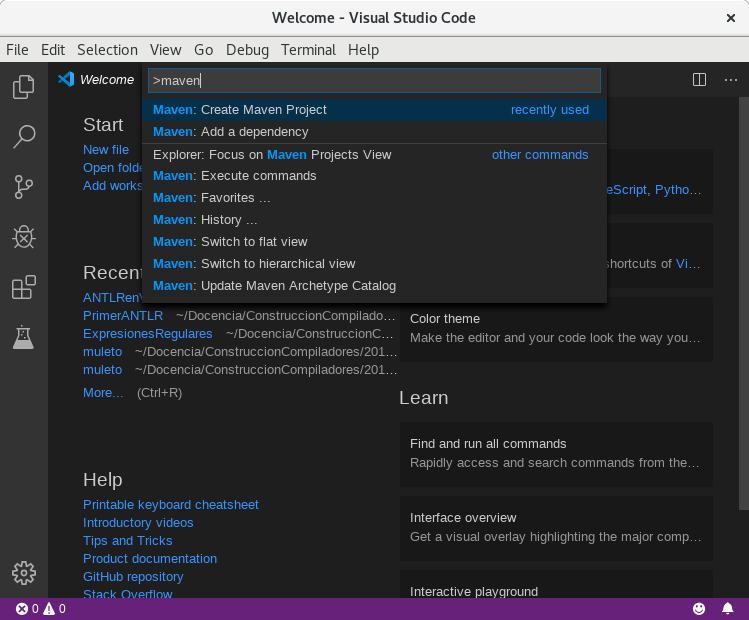
\includegraphics[width=.95\textwidth]{img/CrearMavenProject}
	\caption{Nuevo proyecto Maven.}
	\label{mavenNuevo}
\end{figure}

\begin{figure}[t]
	\centering
	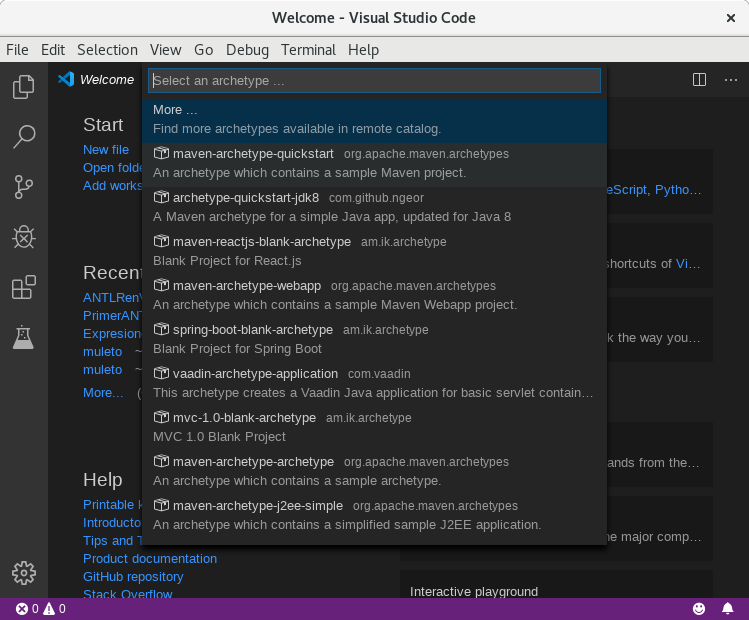
\includegraphics[width=.95\textwidth]{img/MavenArchetypeSample}
	\caption{Arquetipo Maven para Java.}
	\label{mavenArch}
\end{figure}

Finalmente, nos pedirá de forma interactiva en la terminal, que ingresemos datos del proyecto. Se pueden aceptar la mayor parte de la sugerencias, pero lo importante es indicar correctamente el \verb|groupID| y el \verb|artifactID|.  En nuestro caso, usaremos \verb|PrimerProyecto| para ambos campos.  El directorio del proyecto se corresponde con el \verb|groupID|.  Para más información sobre nombres de proyectos ver la documentación en la página de \href{https://maven.apache.org/guides/mini/guide-naming-conventions.html}{Maven}.

\begin{figure}[t]
	\centering
	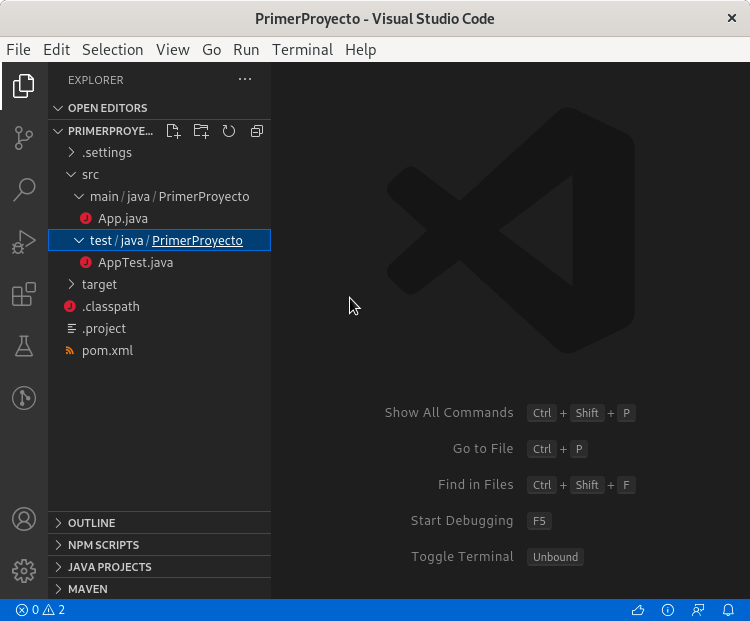
\includegraphics[width=.95\textwidth]{img/MavenProjectoCreado}
	\caption{Proyecto Maven para Java recién creado.}
	\label{mavenSinConf}
\end{figure}

Si el proceso termina correctamente obtendremos un \emph{``Build success''}.  El proyecto no se abre automáticamente, por lo tanto, hay abrirlo desde el menú ``File'' con la opción ``Open Folder'' o usar la combinación de teclas \verb|Ctl+K Ctl+O|.  El proyecto se verá como en la Fig.~\ref{mavenSinConf}.


\subsection{Configuración para Java~11}
\label{mavenJava}

\lstinputlisting[float,style=miXML,caption={Sección \texttt{properties} del archivo \texttt{pom.xml}.},label=pomJava]{code/Java11pom.xml}

Para indicar la versión correcta de Java a usar, debemos editar el archivo \verb|pom.xml|. En la sección \verb|properties| pondremos el número de versión Java como puede verse en el Código~\ref{pomJava}.
    
\begin{figure}[t]
	\centering
	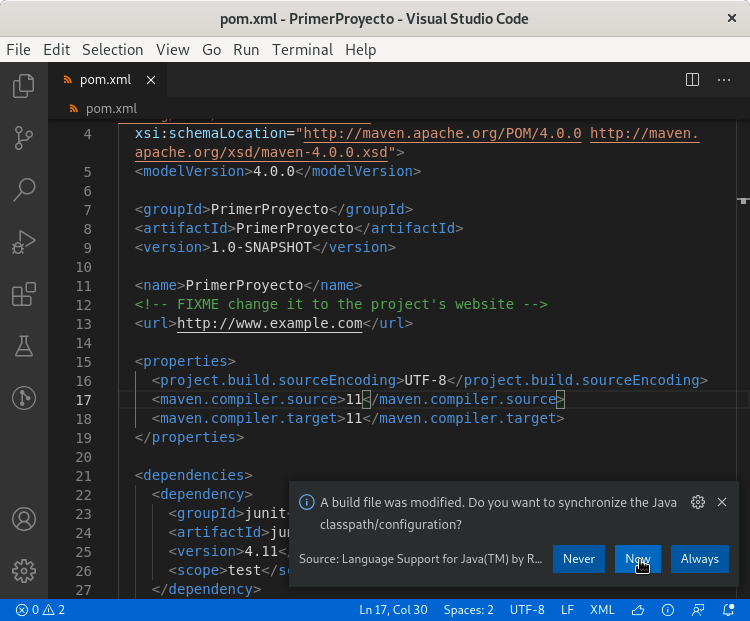
\includegraphics[width=.95\textwidth]{img/MavenPomActualizar}
	\caption{Actualizar configuración proyecto Maven.}
	\label{mavenActConf}
\end{figure}

Al grabar el archivo, se detectará el cambio y preguntará si se desea actualizar la configuración del proyecto (Fig.~\ref{mavenActConf}).  Al aceptar, se podrá ejecutar el proyecto abriendo el archivo \verb|App.java| para verificar la correcta configuración (Fig.~\ref{mavenTestEx}).  Si no encontramos ningún inconveniente, entonces el proyecto se encuentra listo para usar Java~11.


\subsection{Configuración para ANTLR4}
\label{mavenANTLR}

\lstinputlisting[float,style=miXML,caption={Sección \texttt{dependency} del archivo \texttt{pom.xml}.},label=pomANTLR]{code/ANTLRpom.xml}

\begin{figure}[t]
	\centering
	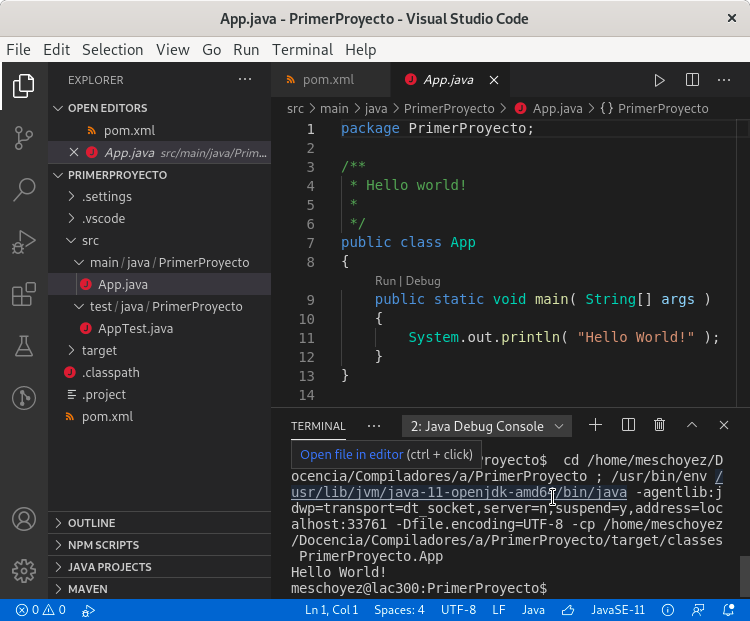
\includegraphics[width=.95\textwidth]{img/MavenTestEx}
	\caption{Prueba configuración del proyecto Maven para Java.}
	\label{mavenTestEx}
\end{figure}

Los gestores de proyectos tienen, entre otros objetivos, resolver las dependencias necesarias para la compilación y ejecución del software con las diferentes bibliotecas de software.  Para usar ANTLR4, debemos configurar su dependencia en el archivo \verb|pom.xml|.  El Código~\ref{pomANTLR} se copió de \href{https://mvnrepository.com/artifact/org.antlr/antlr4}{MVNRepository}.

Finalizados los pasos indicados, tenemos listo el proyecto Maven para compilar en Java un software que utiliza ANTLR4.  En la próxima sección abordaremos como configurar el \emph{plug--in} de ANTLR.


\section{Utilizando ANTLR en el proyecto}
\label{archivo_antlr}

Con el proyecto Java creado y listo para trabajar, vamos a crear un archivo para ANTLR simple. Los archivos de ANTLR llevan extensión \verb|.g| o \verb|.g4|, pero utilizaremos la segunda opción.  El atajo de teclado para crear un archivo vacío es \verb|Ctl+N|, que para hacer efectivo el coloreo hay que guardarlo (\verb|Ctl+S|) con la extensión apropiada.

ANTLR permite la generación del \emph{lexer} y del \emph{parser}.  Por lo tanto, los archivos \verb|.g4| pueden ser para el primero, el segundo o ambos combinados.  Nosotros utilizaremos archivos combinados dentro del paquete que contiene el método \verb|main()| para facilitar la ejecución y visualización de resultados.  En particular, en el proyecto ejemplo guardaremos el archivo \verb|.g4| en la carpeta \verb|src/main/java|.


\subsection{Ejemplo Archivo ANTLR}
\label{ejemplo_archivo_antlr}

A modo de ejemplo, el Código~\ref{id_g4} es un archivo \verb|.g4| del cual se generará el \emph{lexer} y el \emph{parser} que realizan la búsqueda de identificadores tipo Java (nombres de variable, clase o método).  Tanto las reglas léxicas como las gramaticales comienzan con un identificador o etiqueta y terminan en punto y coma (\verb|;|).  Los dos puntos (\verb|:|) indican el comienzo de la regla y la barra vertical o \emph{pipe} (\verb-|-) separan las distintas reglas alternativas.  Las expresiones regulares para la detección de \emph{tokens} se etiquetan con nombres en mayúsculas, como ser \verb|ID| en la línea~10.  Las reglas gramaticales se etiquetan con nombres en minúsculas, como ser \verb|s|.

\lstinputlisting[float,style=miANTLR,caption={Ejemplo de archivo \texttt{.g4}.},label=id_g4]{code/id.g4}

Las palabras reservadas del Código~\ref{id_g4} significan lo siguiente:
\begin{description}
	\item[\texttt{grammar}] Al comienzo del archivo (línea~1) se indica qué queremos generar, siendo \verb|grammar| la palabra reservada tanto para un \emph{parser} como para un archivo combinado. La otra alternativa sería \verb|lexer|.  La palabra \verb|id| es el nombre del \emph{parser}.
	\item[\texttt{@header}] En la línea~3 se utiliza el bloque indicado como \verb|@header| para colocar código fuente en Java que necesitamos que aparezca en todos los código fuente generados por ANTLR.  En el ejemplo se consigna solamente el \verb|package| al que pertenecen.
	\item[\texttt{fragment}] En las líneas~7 y~8 la palabra \verb|fragment| indica que la expresión regular se utilizará para construir expresiones regulares más complejas, por lo tanto, no se utiliza durante el análisis léxico.
\end{description}

Cada vez que se grabe el archivo en disco, el \emph{plug--in} de ANTLR regenerará todos los archivos.



\end{document}
